%!TEX TS-program = xelatex
\documentclass[11pt]{article}

\usepackage[english]{babel}

\usepackage{amsmath,amssymb,amsfonts}
\usepackage[utf8]{inputenc}
\usepackage[T1]{fontenc}
\usepackage{stix2}
\usepackage[scaled]{helvet}
\usepackage[scaled]{inconsolata}

\usepackage{lastpage}

\usepackage{setspace}

\usepackage{ccicons}

\usepackage[hang,flushmargin]{footmisc}

\usepackage{geometry}

\setlength{\parindent}{0pt}
\setlength{\parskip}{6pt plus 2pt minus 1pt}

\usepackage{fancyhdr}
\renewcommand{\headrulewidth}{0pt}\providecommand{\tightlist}{%
  \setlength{\itemsep}{0pt}\setlength{\parskip}{0pt}}

\makeatletter
\newcounter{tableno}
\newenvironment{tablenos:no-prefix-table-caption}{
  \caption@ifcompatibility{}{
    \let\oldthetable\thetable
    \let\oldtheHtable\theHtable
    \renewcommand{\thetable}{tableno:\thetableno}
    \renewcommand{\theHtable}{tableno:\thetableno}
    \stepcounter{tableno}
    \captionsetup{labelformat=empty}
  }
}{
  \caption@ifcompatibility{}{
    \captionsetup{labelformat=default}
    \let\thetable\oldthetable
    \let\theHtable\oldtheHtable
    \addtocounter{table}{-1}
  }
}
\makeatother

\usepackage{array}
\newcommand{\PreserveBackslash}[1]{\let\temp=\\#1\let\\=\temp}
\let\PBS=\PreserveBackslash

\usepackage[breaklinks=true]{hyperref}
\hypersetup{colorlinks,%
citecolor=blue,%
filecolor=blue,%
linkcolor=blue,%
urlcolor=blue}
\usepackage{url}

\usepackage{caption}
\setcounter{secnumdepth}{0}
\usepackage{cleveref}

\usepackage{graphicx}
\makeatletter
\def\maxwidth{\ifdim\Gin@nat@width>\linewidth\linewidth
\else\Gin@nat@width\fi}
\makeatother
\let\Oldincludegraphics\includegraphics
\renewcommand{\includegraphics}[1]{\Oldincludegraphics[width=\maxwidth]{#1}}

\usepackage{longtable}
\usepackage{booktabs}

\usepackage{color}
\usepackage{fancyvrb}
\newcommand{\VerbBar}{|}
\newcommand{\VERB}{\Verb[commandchars=\\\{\}]}
\DefineVerbatimEnvironment{Highlighting}{Verbatim}{commandchars=\\\{\}}
% Add ',fontsize=\small' for more characters per line
\usepackage{framed}
\definecolor{shadecolor}{RGB}{248,248,248}
\newenvironment{Shaded}{\begin{snugshade}}{\end{snugshade}}
\newcommand{\KeywordTok}[1]{\textcolor[rgb]{0.13,0.29,0.53}{\textbf{#1}}}
\newcommand{\DataTypeTok}[1]{\textcolor[rgb]{0.13,0.29,0.53}{#1}}
\newcommand{\DecValTok}[1]{\textcolor[rgb]{0.00,0.00,0.81}{#1}}
\newcommand{\BaseNTok}[1]{\textcolor[rgb]{0.00,0.00,0.81}{#1}}
\newcommand{\FloatTok}[1]{\textcolor[rgb]{0.00,0.00,0.81}{#1}}
\newcommand{\ConstantTok}[1]{\textcolor[rgb]{0.00,0.00,0.00}{#1}}
\newcommand{\CharTok}[1]{\textcolor[rgb]{0.31,0.60,0.02}{#1}}
\newcommand{\SpecialCharTok}[1]{\textcolor[rgb]{0.00,0.00,0.00}{#1}}
\newcommand{\StringTok}[1]{\textcolor[rgb]{0.31,0.60,0.02}{#1}}
\newcommand{\VerbatimStringTok}[1]{\textcolor[rgb]{0.31,0.60,0.02}{#1}}
\newcommand{\SpecialStringTok}[1]{\textcolor[rgb]{0.31,0.60,0.02}{#1}}
\newcommand{\ImportTok}[1]{#1}
\newcommand{\CommentTok}[1]{\textcolor[rgb]{0.56,0.35,0.01}{\textit{#1}}}
\newcommand{\DocumentationTok}[1]{\textcolor[rgb]{0.56,0.35,0.01}{\textbf{\textit{#1}}}}
\newcommand{\AnnotationTok}[1]{\textcolor[rgb]{0.56,0.35,0.01}{\textbf{\textit{#1}}}}
\newcommand{\CommentVarTok}[1]{\textcolor[rgb]{0.56,0.35,0.01}{\textbf{\textit{#1}}}}
\newcommand{\OtherTok}[1]{\textcolor[rgb]{0.56,0.35,0.01}{#1}}
\newcommand{\FunctionTok}[1]{\textcolor[rgb]{0.00,0.00,0.00}{#1}}
\newcommand{\VariableTok}[1]{\textcolor[rgb]{0.00,0.00,0.00}{#1}}
\newcommand{\ControlFlowTok}[1]{\textcolor[rgb]{0.13,0.29,0.53}{\textbf{#1}}}
\newcommand{\OperatorTok}[1]{\textcolor[rgb]{0.81,0.36,0.00}{\textbf{#1}}}
\newcommand{\BuiltInTok}[1]{#1}
\newcommand{\ExtensionTok}[1]{#1}
\newcommand{\PreprocessorTok}[1]{\textcolor[rgb]{0.56,0.35,0.01}{\textit{#1}}}
\newcommand{\AttributeTok}[1]{\textcolor[rgb]{0.77,0.63,0.00}{#1}}
\newcommand{\RegionMarkerTok}[1]{#1}
\newcommand{\InformationTok}[1]{\textcolor[rgb]{0.56,0.35,0.01}{\textbf{\textit{#1}}}}
\newcommand{\WarningTok}[1]{\textcolor[rgb]{0.56,0.35,0.01}{\textbf{\textit{#1}}}}
\newcommand{\AlertTok}[1]{\textcolor[rgb]{0.94,0.16,0.16}{#1}}
\newcommand{\ErrorTok}[1]{\textcolor[rgb]{0.64,0.00,0.00}{\textbf{#1}}}
\newcommand{\NormalTok}[1]{#1}

\newlength{\cslhangindent}
\setlength{\cslhangindent}{1.5em}
\newlength{\csllabelwidth}
\setlength{\csllabelwidth}{3em}
\newenvironment{CSLReferences}[3] % #1 hanging-ident, #2 entry spacing
 {% don't indent paragraphs
  \setlength{\parindent}{0pt}
  % turn on hanging indent if param 1 is 1
  \ifodd #1 \everypar{\setlength{\hangindent}{\cslhangindent}}\ignorespaces\fi
  % set entry spacing
  \ifnum #2 > 0
  \setlength{\parskip}{#2\baselineskip}
  \fi
 }%
 {}
\usepackage{calc} % for \widthof, \maxof
\newcommand{\CSLBlock}[1]{#1\hfill\break}
\newcommand{\CSLLeftMargin}[1]{\parbox[t]{\maxof{\widthof{#1}}{\csllabelwidth}}{#1}}
\newcommand{\CSLRightInline}[1]{\parbox[t]{\linewidth}{#1}}
\newcommand{\CSLIndent}[1]{\hspace{\cslhangindent}#1}\geometry{verbose,letterpaper,tmargin=2.2cm,bmargin=2.2cm,lmargin=2.2cm,rmargin=2.2cm}

\usepackage{lineno}
\usepackage[nolists,noheads]{endfloat}

\pagestyle{plain}

\tolerance=1
\emergencystretch=\maxdimen
\hyphenpenalty=10000
\hbadness=10000

\doublespacing

\fancypagestyle{normal}
{
  \fancyhf{}
  \fancyfoot[R]{\footnotesize\sffamily\thepage\ of \pageref*{LastPage}}
}
\begin{document}
\raggedright
\thispagestyle{empty}
{\Large\bfseries\sffamily Thesis proposal}
\vskip 5em

%
\href{https://orcid.org/0000-0002-6506-6487}{Michael D.\,Catchen}%
%
\,\textsuperscript{1,2}

\textsuperscript{1}\,McGill University\quad \textsuperscript{2}\,Québec
Centre for Biodiversity Sciences


\textbf{Correspondance to:}\\
Michael D. Catchen --- \texttt{michael.catchen@mail.mcgill.ca}\\

\vfill
This work is released by its authors under a CC-BY 4.0 license\hfill\ccby\\
Last revision: \emph{\today}

\clearpage
\thispagestyle{empty}

\vfill
The proposal for my thesis, \emph{Simulation models for predictive
ecology}



\vfill

\clearpage
\linenumbers
\pagestyle{normal}

\hypertarget{introduction}{%
\section{Introduction}\label{introduction}}

\begin{longtable}[]{@{}l@{}}
\toprule
\endhead
\begin{minipage}[t]{0.05\columnwidth}\raggedright
\textbf{P1}\strut
\end{minipage}\tabularnewline
\begin{minipage}[t]{0.05\columnwidth}\raggedright
Within the last several hundred years, human activity have rapidly
changed Earth's atmosphere, oceans, and surface. Greenhouse gas
emissions have caused an increase the temperature of both Earth's
surface and oceans (resulting in acidification), and both agricultural
and urban development has rapidly reshaped Earth's surface. These the
bulk of this change has occurred within the last several hundred years,
a geological instant, potentially inducing shocks to ecosystems that
could threated their integrity (\textbf{Scheffer?}). As a result
understanding and predicting how ecosystems will change in the future,
\emph{ecological forecasting}, and making making descisions based on
these predictions mitigating the consequences of this change, on
ecosystems has emerged as an imperative for ecology and environmental
science {[}Dietze (2017);{]}.\strut
\end{minipage}\tabularnewline
\bottomrule
\end{longtable}

\textbf{P2}

However, robust forecasting of ecological processes will change in the
future is, to say the least, quite difficult. This difficultly is
compounded by a few factors, the first being that sampling ecosystems is
not easy. Ecological data is often biased, and noisey, spatially and
temporally sparse. As a result \emph{ecosystem monitoring} (Makiola
\emph{et al.} 2020) has emerged as an imperative. Developing a system
for ecological observation, which is able to coordinate across
locations. (\textbf{AndyUrbanBiomonitoring?} paper).

\begin{center}\rule{0.5\linewidth}{0.5pt}\end{center}

The second major challenge in forecasting ecosystems is that the
underlying dynamics of most ecological processes are fundementally
unknown (and unknowable) and instead must be inferred.

Much of the history of quantitatively modeling ecosystems have been done
in the language of dynamical systems, describing how the value of an
observable state of the system, represented by a vector of numbers
\([x_1, x_2, \dots, x_n]^T = \vec{x}\) changes as over time. It turns
out to be much more effective to, rather than attempt to directly model
\(\vec{x}(t)\) itself, to instead describe how \(\vec{x}\) changes from
one timestep to the next, yielding models in the form of differential
equations in continuous-time settings--\(\frac{dx}{dt} = f(x)\)-- or
difference equations in discrete-time
settings---\(x_t = f(x_{t-1})\)---where
\(f:\mathbb{R}^n \to \mathbb{R}^n\) is an arbitrary function describing
how the system changes on a moment-to-moment basis (e.g.~in the context
of communities, \(f\) could be Lotka-Voltera, Holling-Type-III or
DeAngelis-Beddington functional response). The form of this functional
response in real systems is effectively unknown, and some forms are
inherently more ``forecastable'' than others (Chen \emph{et al.} 2019).

\begin{longtable}[]{@{}l@{}}
\toprule
\endhead
\begin{minipage}[t]{0.05\columnwidth}\raggedright
\textbf{P3}\strut
\end{minipage}\tabularnewline
\begin{minipage}[t]{0.05\columnwidth}\raggedright
However, we run into many problems when aiming to apply this type of
model to empirical data in ecology.\strut
\end{minipage}\tabularnewline
\begin{minipage}[t]{0.05\columnwidth}\raggedright
The initial success of ODE models can be traced back to the larger
program of ontological reductionism, which became the de facto apporoach
model physical sciences after its early success in physics, which, and
by the time ecology was becoming a quantitative science (sometime in the
20th century, depending on who you ask), became the foundation for early
quantitative models in ecology.\strut
\end{minipage}\tabularnewline
\begin{minipage}[t]{0.05\columnwidth}\raggedright
But ecosystems are perhaps the quintessential example of system that
cannot be understood simply by iterative reduction of its components.
Emergent phenomena, mechanisms at different scales, etc.\strut
\end{minipage}\tabularnewline
\begin{minipage}[t]{0.05\columnwidth}\raggedright
Some have been explored in the ecological literature: (1) Some
applications of dynamic models in ecology assume long-run equilibrium.
(2) Stochasticity\strut
\end{minipage}\tabularnewline
\begin{minipage}[t]{0.05\columnwidth}\raggedright
(3) Ecological processes vary across more variables than the tools of
analytic models are suited for. As the number of variables in an
analytic model increases, so does the ability of the scientist to decern
clear relationships between them, and so does overfitting potential.
Curse of dimensionality--- Until the 20th century, no theory of the
gravitational dynamics of more than 2 bodies. Understanding the
gravitational dynamics of more than two planets with any reliability
proved difficult. Using the same models (diffeqs), how could we
adequately predict ecosystems?\strut
\end{minipage}\tabularnewline
\bottomrule
\end{longtable}

\emph{P4}

The term \emph{ecological forecasting} implicitly creates an analogy
between predicting how ecosystems will change in the future by using the
term ``forecasting''---the most immediate analog being the success story
of weather forecasting via numerical weather prediction (NWP).

Although it is become almost hack to complain about the dang weather
forecast being wrong, over the least 50 years the
(\textbf{Bauer2015QuiRev?}).

The success of NWP, and the Earth observations that support it should
serve as a template for development of a system for monitoring Earth's
biodiversity. Much like ecology, NWP is faced with high-dimensional
systems that are governed by different mechanisms at different scales.

Much as one would not aim to forecast the weather in Quebec by applying
Navier-Stokes. NWP has worked because it incorporates information about
data and meteorological processes collected at difference scales into
models that. Use of computational methods in NWP.

Transition to simulation as the solution: shift toward approach of
building models that \emph{generate} data.

(resolving the semantic ambuity of what differentiates ``mechanistic''
vs ``phenomological'' models is out of scope for now).

More broadly a reflection reflect ecology lagging behind the statistical
methods used in sciences that face similar challenges (many dimensions,
many mechanisms at different scales, each with stochasticity). Chaotic
dynamics emerge from simple analytic models, and . Whether ecosystems
actually exhibit chaotic behavior is a different question.

\begin{longtable}[]{@{}l@{}}
\toprule
\endhead
\begin{minipage}[t]{0.07\columnwidth}\raggedright
\textbf{P5}\strut
\end{minipage}\tabularnewline
\begin{minipage}[t]{0.07\columnwidth}\raggedright
But forecasting isn't the only difficult problem here.\strut
\end{minipage}\tabularnewline
\begin{minipage}[t]{0.07\columnwidth}\raggedright
Transition to theme of optimization given unknown information. A
forecast gives us a range of future values with uncertainty around them.
Further a convenient property that a forecasting model's uncertainty
goes up over time (if we assume the underlying process is Markov--this
is a strong assumption but oft true of the models we fit to temporal
data)\strut
\end{minipage}\tabularnewline
\begin{minipage}[t]{0.07\columnwidth}\raggedright
In face of uncertainty, decision making is an optimization problem. We
have some goal state for the future, and some estimate of what the state
of the world will be given a set of actions. Frame optimization problem
mathematically an introduce concept of solution-space and
constraint.\strut
\end{minipage}\tabularnewline
\begin{minipage}[t]{0.07\columnwidth}\raggedright
Indeed Marx's most well known quote that ``philosophers have hitherto
only interpreted the world in various ways; the point is to change
it.''\strut
\end{minipage}\tabularnewline
\begin{minipage}[t]{0.07\columnwidth}\raggedright
and a necessary step toward establishing a just and sustainable
world.\strut
\end{minipage}\tabularnewline
\bottomrule
\end{longtable}

\begin{figure}
\hypertarget{fig:thesis}{%
\centering
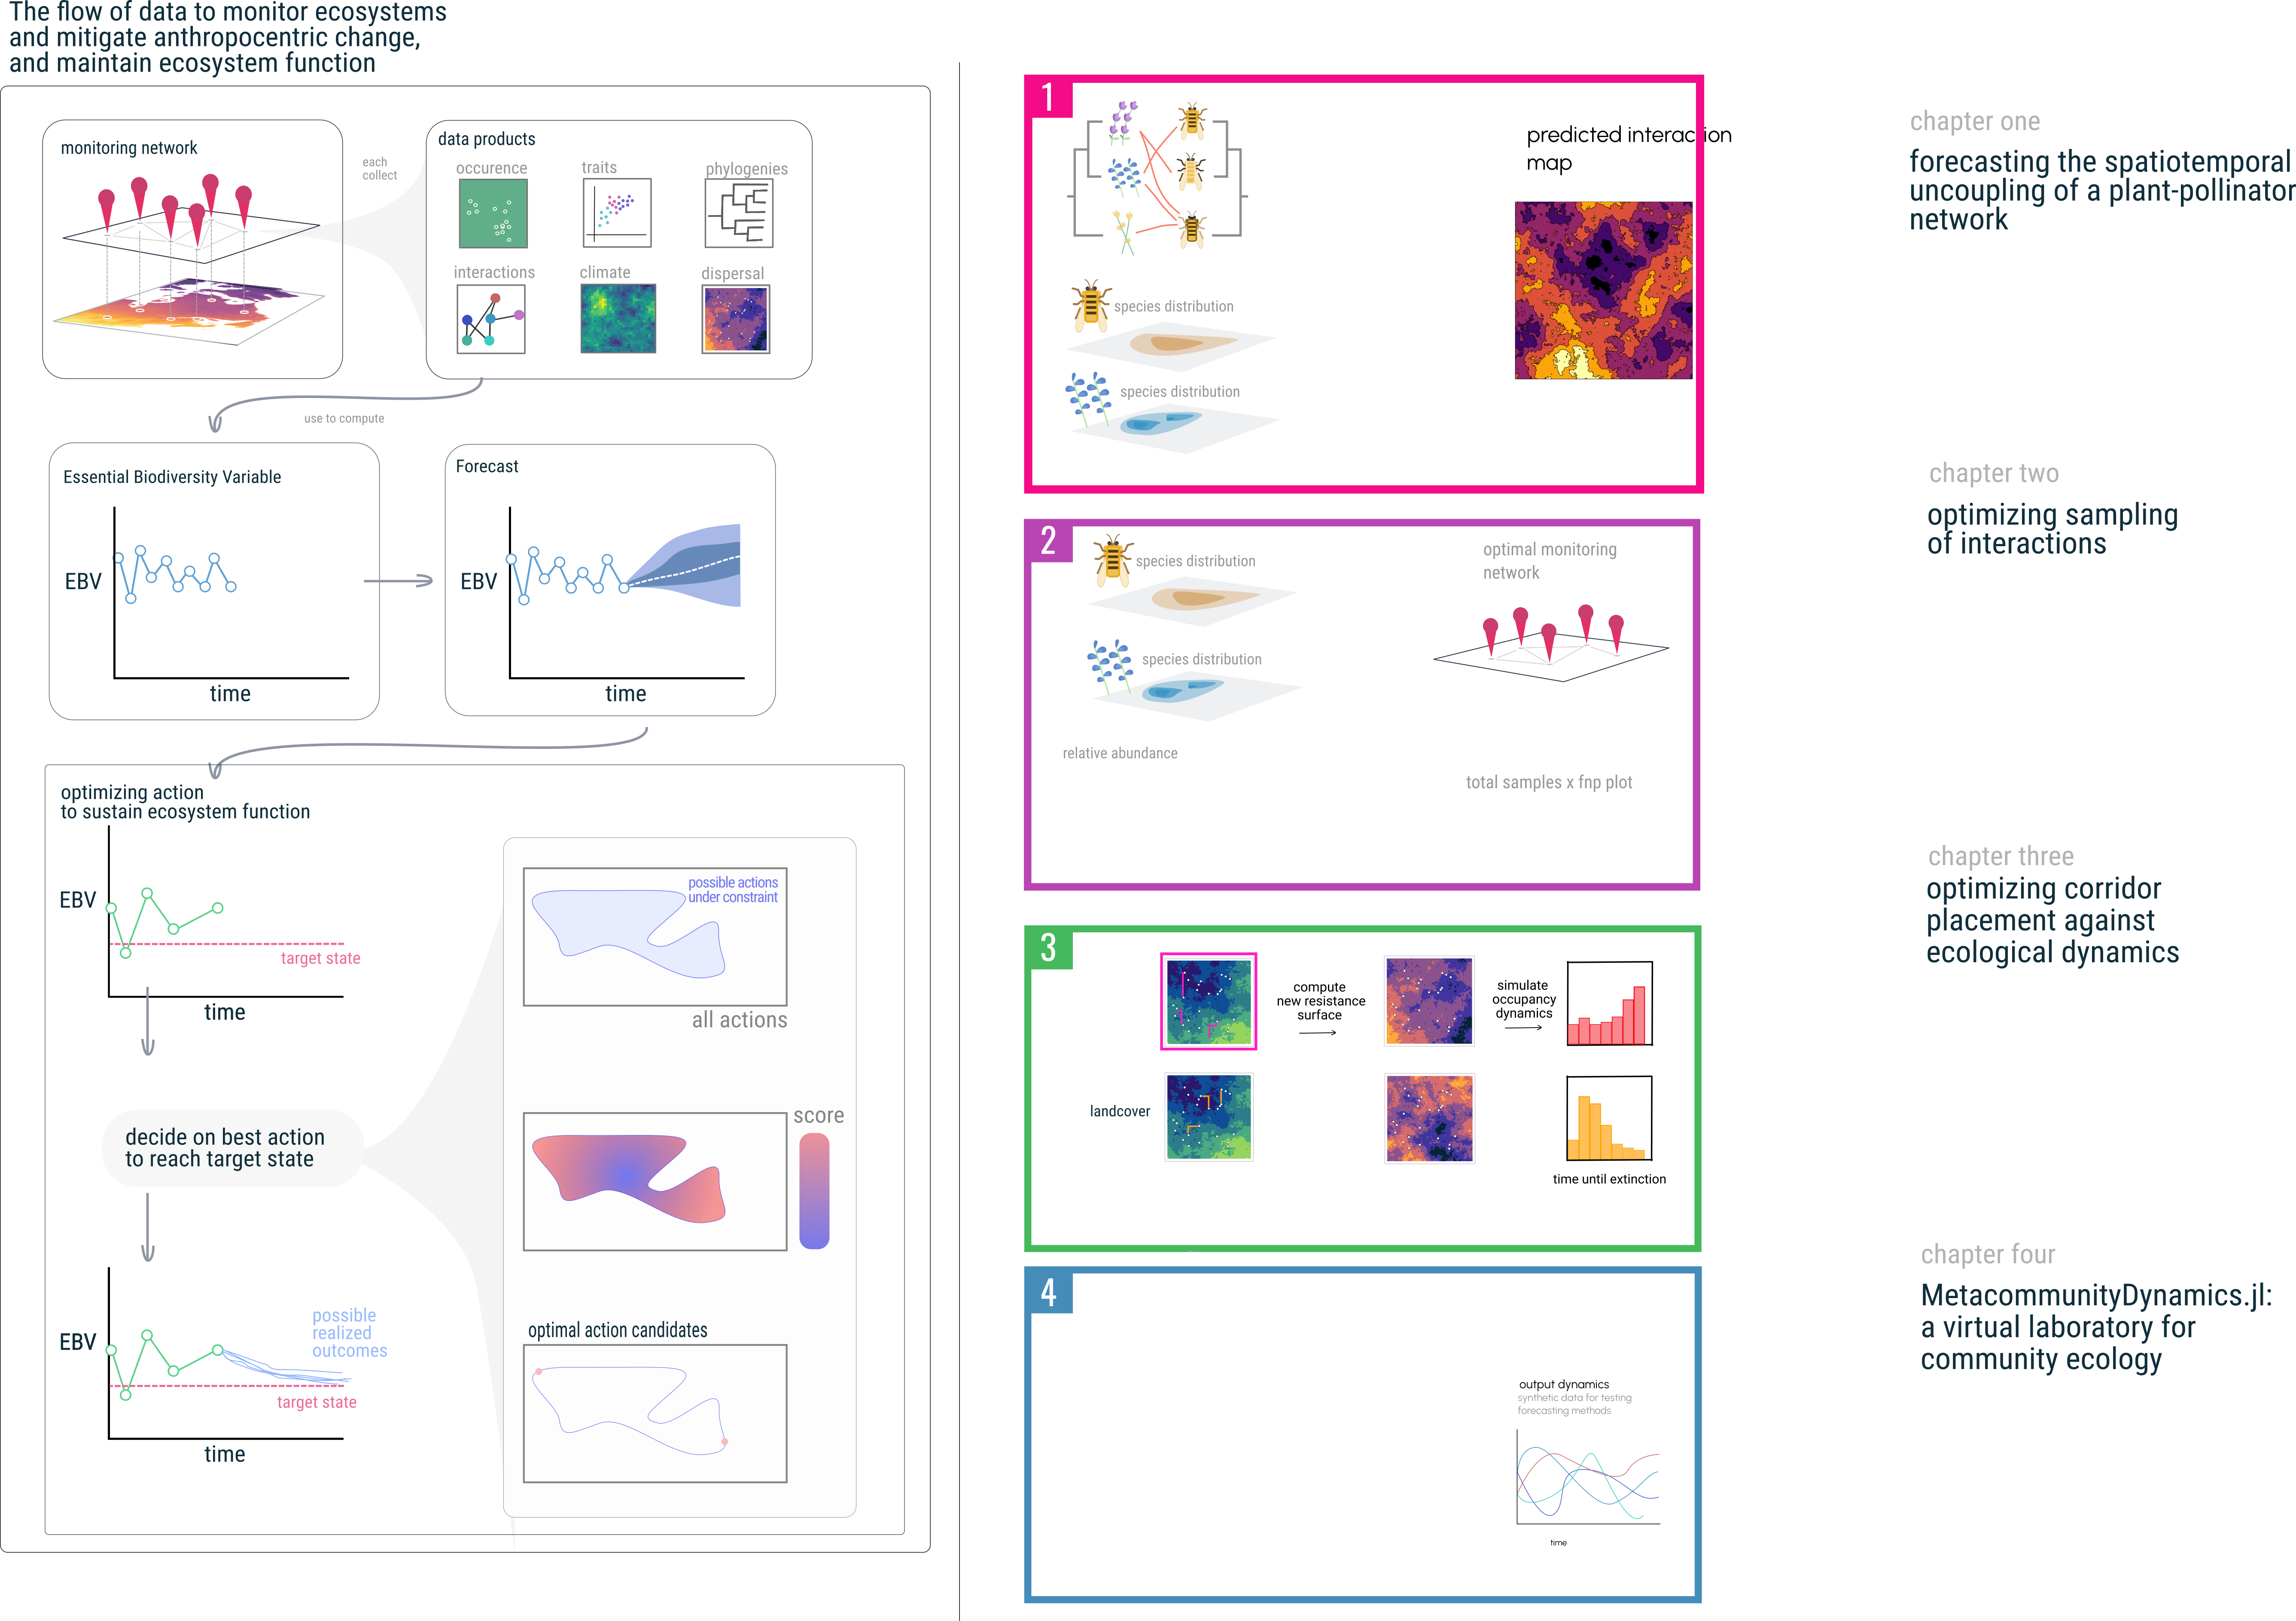
\includegraphics{./figures/thesisconcept.png}
\caption{thesis concept}\label{fig:thesis}
}
\end{figure}

\textbf{P6 -- final intro para}

Three major components here: 1) Ecosystem monitoring, 2) Forecasting
using the products of that monitoring, and 3) Choosing the best possible
mitigation strategy.

This flow is outlined in the left panel of fig.~\ref{fig:thesis}

\hypertarget{chapter-one-forecasting-the-spatial-uncoupling-of-a-plant-pollinator-network}{%
\section{Chapter One: Forecasting the spatial uncoupling of a
plant-pollinator
network}\label{chapter-one-forecasting-the-spatial-uncoupling-of-a-plant-pollinator-network}}

Plants and pollinators form interaction networks, called the
``architecture of biodiversity'' (\textbf{Jordano2007?}).

The stability, function, and persistance of ecosystems relies on the
structure of these interactions. Antropogenic change threatens to
unravel these networks. Two aspects to this change: spatial and
temporal. Spatially, range shifts along elevational gradient, and
temporall, phenological shifts.

The issue is that we don't really know what interactions are like now.
So not only do we need to predict with data that is spatially and
temporally sparse and likely to contain many interaction
``false-negatives'' (\textbf{Strydom2021?})

This chapter uses several years of data on bee-flower phenology and
interactions, combined with spatial records of species occurrence via
GBIF, to forecast how much overlap there will be between
plants/pollinators in space/time.

In stages, (1) take data from multiple sites to predict a spatial
metaweb of \emph{Bombus}-flower interactions across Colorado. (2)
Predict how these spatial distributions will change under CMIP6. and (3)
quantify the lack of overlap between species for which there is a
predicted

\textbf{CH1 concept figure}

\hypertarget{data}{%
\subsection{Data}\label{data}}

System description: lots of data on \emph{Bombus} (bumblebees) and
wildflowers. Three different sites, (7/7/3) years each, each covering an
elevational gradient.

\hypertarget{methods}{%
\subsection{Methods}\label{methods}}

Split the process into parts.

\begin{enumerate}
\def\labelenumi{\arabic{enumi})}
\tightlist
\item
  Building an interaction prediction model.
\item
  Make it spatial based on distributions.
\item
  Forecast distributions based on CMIP6.
\end{enumerate}

\hypertarget{preliminary-results}{%
\subsection{Preliminary Results}\label{preliminary-results}}

\begin{enumerate}
\def\labelenumi{\arabic{enumi})}
\tightlist
\item
  we got a tree
\end{enumerate}

Transition to next chapter by discussing uncertainty in interaction
prediction across space.

\hypertarget{ch2-optimizing-sampling-of-interactions}{%
\section{CH2 optimizing sampling of
interactions}\label{ch2-optimizing-sampling-of-interactions}}

This chapter quantifies the relationship between a given species
relative abundance and the sampling effort needed to adequately
understand this species distribution and interactions.

For a given sample of interaction data, and proposes a method for
optimizing spatial sampling of a possible interaction between species as
a function of the estimated distribution of both species.

\hypertarget{methods-1}{%
\subsection{Methods}\label{methods-1}}

\begin{itemize}
\item
  the missing link paper, turn this into optimizing with two different
  SDMs
\item
  relative abundance and its effect on false negative
\item
  non-independent associations in samples
\item
  simulate species distribution and efficacy of detection given a set of
  observation points where the dist from observation site decays.
\item
  optimize set of repeated sampling locations L for a \emph{known}
  distribution D.
\item
  address SDM not being the territory
\end{itemize}

\hypertarget{results}{%
\subsection{Results}\label{results}}

\hypertarget{in-progress-results}{%
\subsubsection{In-progress results}\label{in-progress-results}}

\hypertarget{ch3-optimizing-corridor-placement}{%
\section{CH3 optimizing corridor
placement}\label{ch3-optimizing-corridor-placement}}

This chapter proposes an algorithm for optimizing restoration across
space

(corridorplacement/restoration effort) given a raster where each cell
indicates land-cover. The optimization method uses the result of a
simulated process (specifically occupancy dynamics in the landscape) and
uses simulated annealing to estimate the global optimum of the
targetstate (specfically mean-time-to-extinction for the occupancy
dynamics example).

\hypertarget{methods-2}{%
\subsection{Methods}\label{methods-2}}

\begin{itemize}
\tightlist
\item
  land cover -\textgreater{} resistance -\textgreater{} extinction time
\item
  simulated annealing to optimize landscape optimization
\end{itemize}

\hypertarget{ch4-a-software-note-on-the-resulting-packages.}{%
\section{CH4 a software note on the resulting
packages.}\label{ch4-a-software-note-on-the-resulting-packages.}}

(MetacommunityDynamics.jl: a virtual laboratory for community ecology):
a collection of modules in the Julia language for different aspects of
metacommunity ecology, including most of the code used for the preceding
chapters.

\begin{itemize}
\item
  TK conceptual figure with interfaces between what I'm writing / have
  contributed to and linked with other libraries
\item
  \texttt{Observatories.jl}, \texttt{Corridors.jl}, \texttt{MCD.jl}
\end{itemize}

\hypertarget{concl}{%
\section{concl}\label{concl}}

// this is a discussion para An oft applied definition of the origin of
is ``the application of the scientific method to natural history.''
Since its origin ecology has been a descriptive science. This is a
natural by-product of the immense variability of Earth's biosphere.
emerged to explain particular phenomena at particular scales. In recent
years, there has been an interest in an epistemological shift in
ecology. To shift ecology into a predictive science. The justification
for this shift is twofold: (1) bogged down philosophy of science, by
further rooting our understanding of ecosystem function and dynamics in
an ability to predict their structure (Dietze 2017). and (2) the
practical need for models for \emph{ecological forecasting}.

\hypertarget{references}{%
\section*{References}\label{references}}
\addcontentsline{toc}{section}{References}

\hypertarget{refs}{}
\begin{CSLReferences}{1}{0}
\leavevmode\hypertarget{ref-Chen2019RevCom}{}%
Chen, Y., Angulo, M.T. \& Liu, Y.-Y. (2019). Revealing Complex
Ecological Dynamics via Symbolic Regression. \emph{BioEssays}, 41,
1900069.

\leavevmode\hypertarget{ref-Dietze2017PreEco}{}%
Dietze, M.C. (2017). Prediction in ecology: A first-principles
framework. \emph{Ecological Applications}, 27, 2048--2060.

\leavevmode\hypertarget{ref-Makiola2020KeyQue}{}%
Makiola, A., Compson, Z.G., Baird, D.J., Barnes, M.A., Boerlijst, S.P.,
Bouchez, A., \emph{et al.} (2020). Key Questions for Next-Generation
Biomonitoring. \emph{Frontiers in Environmental Science}, 7.

\end{CSLReferences}

\end{document}
